\chapter{机器人驱动器}
\label{chap:actuators}

\begin{focusbox}{本章复习路线}
驱动器把电能、液压能或气动能转换为关节的机械功。复习时沿着\textbf{电流产生转矩、转速产生反电动势、传动改变关节转速和转矩}这条线推导。给定一项关节动作，要能从关节需求算到电机工作点，并说明转速、峰值转矩和连续发热分别由什么限制。
\end{focusbox}

\section{驱动单元与驱动方式}

机器人驱动单元通常由动力源、功率放大器或驱动器、执行元件及传动机构组成。控制器输出指令，功率放大器按指令调节供给执行元件的功率，电机、液压缸或气缸产生机械运动，传动机构再将运动和转矩送至关节。旋转系统的机械功率为 $P=\tau\omega$，直线系统为 $P=Fv$。

\begin{figure}[htbp]
\centering
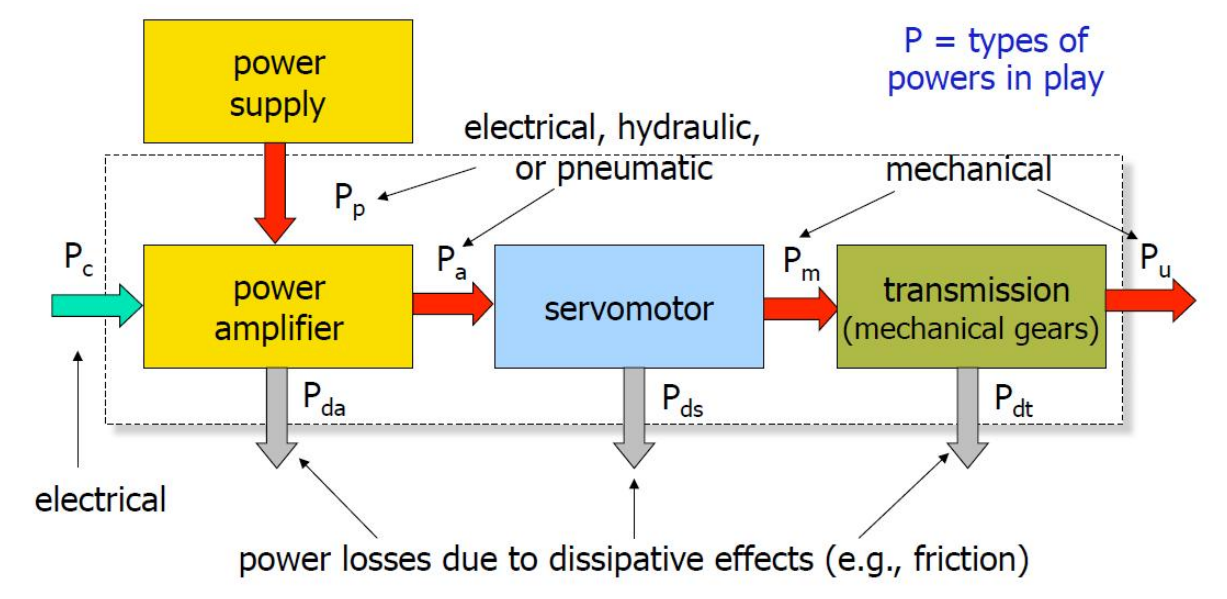
\includegraphics[width=.78\linewidth]{01-actuation-system.png}
\caption{动力源、功率放大器、执行元件和传动装置。取自《Actuators》PDF 第24页。}
\label{fig:actuation-system}
\end{figure}

\begin{table}[htbp]
\centering\small
\begin{tabularx}{\linewidth}{@{}l X X@{}}
\toprule
方式 & 工作特点 & 选型与应用 \\
\midrule
电动 & 电机由电压、电流驱动，便于与编码器组成精确伺服。电机通电保持负载时会产生铜损。 & 常见于工业机器人关节。校核发热、供电和制动保持需求。 \\
液压 & 由压力液体驱动液压缸或马达，可在低速下输出很大的力或转矩。 & 适合重载。需油源与阀组，并考虑泄漏、维护和系统体积。 \\
气动 & 压缩空气驱动，结构可较简单，气体压缩性使系统具有柔顺性。 & 适合开合与简单往复，如夹爪。负载变化时，精确轨迹控制较难。 \\
\bottomrule
\end{tabularx}
\end{table}

\textbf{机器人关节的典型要求}包括高功率重量比、低惯量、启停与换向能力、宽速域和低速平稳性。定位准确度看实际位置偏离目标的程度，重复定位精度看相同命令下位置的离散程度。

\FloatBarrier
\section{永磁直流电机的机电模型}

\subsection{洛伦兹力与换向}

均匀磁场中，一段方向沿电流的导线 $\boldsymbol{\ell}$ 受到 $\boldsymbol{F}=i_a\boldsymbol{\ell}\times\boldsymbol{B}$。矩形线圈两侧的电流方向相反，磁场力也相反，形成力偶。用 $d$ 表示每侧距转轴的距离，按图\ref{fig:actuator-commutation}的角度约定，单匝有效力臂为 $d\cos\theta$，转矩大小随角度按 $2d|F\cos\theta|$ 变化。为了连续转动，有刷直流电机利用电刷与换向器在转子转过相应位置时改变线圈电流方向，使转矩保持同向。多绕组错相布置可减小转矩脉动。

\begin{figure}[htbp]
\centering
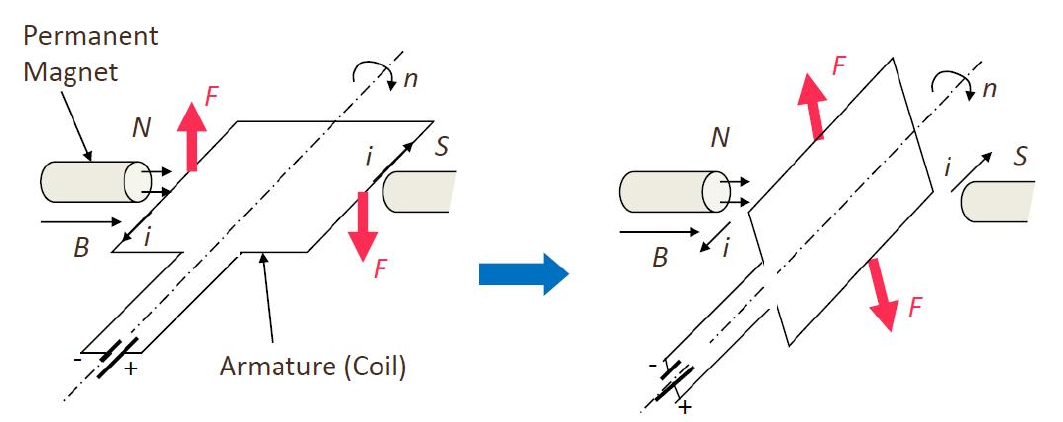
\includegraphics[width=.79\linewidth]{01-dc-motor-commutation.png}
\caption{线圈两侧的磁场力及其力臂。取自《Actuators》PDF 第7页的示意图。}
\label{fig:actuator-commutation}
\end{figure}

\subsection{电路、转矩与机械运动}
\label{sec:actuator-equations}

设电枢电压 $u$、电流 $i_a$、电阻 $R$、电感 $L$，电机角速度 $\omega_m$，电磁转矩 $\tau_e$。取电压、电流和转矩的正方向一致，并把折算到电机轴的外部负载转矩 $\tau_L$ 定为正转时的阻转矩。线性模型为
\begin{align*}
 u &= Ri_a+L\frac{\mathrm di_a}{\mathrm dt}+e_b,
 & e_b&=K_e\omega_m,\\
 \tau_e&=K_t i_a,
 &J\frac{\mathrm d\omega_m}{\mathrm dt}+B\omega_m&=\tau_e-\tau_L .
\end{align*}
这里 $J$ 是按所选轴折算的惯量，$B$ 为黏性阻尼系数。若 $J$ 已含负载惯量，$\tau_L$ 只计其余阻转矩。反电动势由转子旋转产生，在正向电动工况中压低同电压下的电流。乘以电流可写成
\[
ui_a=Ri_a^2+\frac{\mathrm d}{\mathrm dt}\left(\frac12 Li_a^2\right)+e_bi_a.
\]
理想机电转换满足 $e_bi_a=\tau_e\omega_m$，故在 $K_t$ 用 $\mathrm{N\,m/A}$、$K_e$ 用 $\mathrm{V\,s/rad}$ 时，两者数值相等。若手册给出 $\mathrm{rpm/V}$ 的速度常数 $K_v$，转为上述单位应取 $K_e=60/(2\pi K_v)$。零初值下令 $\tau_L=0$，消去电流，可得电压到角速度的模型
\[
\frac{\Omega_m(s)}{U(s)}=\frac{K_t}{(Ls+R)(Js+B)+K_tK_e}.
\]
固定转子时，电流的一阶时间常数为 $L/R$。忽略电枢电感时，角速度的一阶时间常数为 $J/(B+K_tK_e/R)$，角位置模型再乘 $1/s$。

\nt{\textbf{建模条件}　稳态电流允许略去 $L\,\mathrm di_a/\mathrm dt$，瞬态电流响应要保留电感。手册中绕组温度变化会改变 $R$，精细选型需使用相应温度下的工作参数。}

\FloatBarrier
\section{矩速曲线与参数表}

在恒定端电压 $U$ 下，取稳态并忽略机械损耗，$\tau=\tau_e$，从 $U=R\tau/K_t+K_e\omega$ 得
\[
\boxed{\omega=\frac{U}{K_e}-\frac{R}{K_e K_t}\tau},\qquad
\omega_0=\frac{U}{K_e},\qquad \tau_s=K_t\frac{U}{R}.
\]
$\omega_0$ 是理想空载转速，$\tau_s$ 是理想堵转转矩。在实际电机中，空载仍需小电流克服摩擦等损耗，实际空载转速略低于上述理想值。在这个模型和端电压下，轴机械功率为
\[
P_{\mathrm{out}}=\tau\omega=\omega_0\tau\left(1-\frac{\tau}{\tau_s}\right),\qquad
P_{\max}=\frac{\tau_s\omega_0}{4}
\quad\text{当 }\tau=\frac{\tau_s}{2},\ \omega=\frac{\omega_0}{2}.
\]
堵转和理想空载的轴输出功率都为零。堵转仍可能伴随很大的电流和温升；在此理想模型中，最大机械功率点的效率为 $1/2$，等于该点反电动势与端电压的比值。

\begin{figure}[htbp]
\centering
\begin{tikzpicture}
\begin{axis}[
  width=.74\linewidth,height=4.45cm,xmin=0,xmax=1.08,ymin=0,ymax=1.19,
  axis lines=left, xlabel={$\tau/\tau_s$}, ylabel={归一化值},
  xtick={0,.5,1},xticklabels={$0$,$1/2$,$1$},
  ytick={0,.5,1},yticklabels={$0$,$1/2$,$1$},
  legend style={at={(.5,1.03)},anchor=south,legend columns=2,draw=none,font=\small}]
\addplot[myb,very thick,domain=0:1] {1-x};
\addlegendentry{$\omega/\omega_0$}
\addplot[myr,very thick,dashed,domain=0:1,samples=50] {4*x*(1-x)};
\addlegendentry{$P_{\mathrm{out}}/P_{\max}$}
\draw[densely dotted,gray] (axis cs:.5,0)--(axis cs:.5,1);
\end{axis}
\end{tikzpicture}
\caption{恒压条件下的理想矩速曲线和机械功率曲线。依据《Actuators》PDF 第14页重绘。}
\label{fig:actuator-torque-speed}
\end{figure}

\textbf{读电机参数表时先认运行条件。}额定功率对应指定工况。连续转矩受温升限制，峰值转矩还受驱动限流和持续时间限制。最大机械功率点、最大效率点与额定点各有定义。电机常数 $K_m=K_t/\sqrt R$，同转矩下可用 $P_{\mathrm{Cu}}=\tau_e^2/K_m^2$ 比较铜损。

\ex{由端电压求工作点}{设 $U=24\,\mathrm V$、$R=2\,\Omega$、$K_t=0.10\,\mathrm{N\,m/A}$、$K_e=0.10\,\mathrm{V\,s/rad}$。忽略机械损耗，稳态负载转矩为 $0.30\,\mathrm{N\,m}$。求电流、转速、轴功率，并检验功率平衡。}

\textbf{解}　先按转矩算电流，再按电压平衡求转速。
\[
i_a=\frac{0.30}{0.10}=3.0\,\mathrm A,\qquad
\omega=\frac{24-2\times3}{0.10}=180\,\mathrm{rad/s}.
\]
机械输出为 $0.30\times180=54\,\mathrm W$；电输入 $24\times3=72\,\mathrm W$，铜损 $3^2\times2=18\,\mathrm W$。两项相加等于输入功率。由曲线截距公式得 $\tau_s=1.2\,\mathrm{N\,m}$、$\omega_0=240\,\mathrm{rad/s}$，理想最大轴功率为 $72\,\mathrm W$。

\FloatBarrier
\section{传动与关节负载折算}
\label{sec:actuator-transmission}

\textbf{减速比与传动效率}　取减速比 $N=\omega_m/\omega_j>1$，电机向负载供能时，若传动效率为 $\eta$，有
\[
\boxed{\omega_j=\omega_m/N,\qquad \tau_j=\eta N\tau_m},\qquad
P_j=\eta P_m .
\]
下标 $m,j$ 分别为传动输入电机侧和输出关节侧。机构反转时须另计旋向。

由齿轮、同步带或其他机构实现减速增扭；丝杠可将旋转变为平移。若丝杠导程 $p$ 指一转的轴向位移，则前向驱动时 $v=p\omega/(2\pi)$；以效率 $\eta$ 和功率平衡计算推力 $F=2\pi\eta\tau/p$。传动还能把电机布置在靠近基座处，以减轻运动部件，但要考虑间隙、摩擦和柔性。

\textbf{惯量折算由动能决定。}忽略传动件自身惯量，负载惯量 $J_j$ 的动能为
\[
\frac12 J_j\omega_j^2=\frac12 \frac{J_j}{N^2}\omega_m^2.
\]
因此 $J_j$ 折算至电机轴为 $J_j/N^2$；反过来，电机转子惯量 $J_m$ 折算至关节为 $N^2J_m$。前向传动的效率用于按功率折算转矩，动能等效本身由速度比决定。较高减速比可减小电机轴所见负载惯量，同时增大关节所见转子惯量，并提高相同关节速度所要求的电机转速。

电机选型时，可据力臂和加速度求关节转矩，再按传动关系映射到电机。比较具体工作点的可用转矩和转速；有重复工作周期且铜损占主导时，用 $\tau_{\mathrm{rms}}=\sqrt{\sum_k\tau_k^2\Delta t_k/\sum_k\Delta t_k}$ 初估发热，另行校核峰值、散热和实际矩速包络。

\ex{减速器与电机轴的需求}{关节负载惯量 $J_j=0.18\,\mathrm{kg\,m^2}$，运动时有恒定阻转矩 $5.0\,\mathrm{N\,m}$。关节从静止以恒加速度在 $0.20\,\mathrm s$ 内达到 $1.20\,\mathrm{rad/s}$。传动比 $N=12$、前向效率 $\eta=0.90$，电机转子惯量 $J_m=0.002\,\mathrm{kg\,m^2}$。忽略其他惯量和损耗，求加速阶段所需的电磁转矩和阶段末转速。}

\textbf{解}　关节角加速度为 $6.0\,\mathrm{rad/s^2}$，所需输出转矩为 $5.0+0.18\times6.0=6.08\,\mathrm{N\,m}$。电机轴传入减速器的转矩为 $6.08/(0.90\times12)=0.563\,\mathrm{N\,m}$，电机转子另需 $J_mN\alpha_j=0.144\,\mathrm{N\,m}$，故
\[
\tau_e\approx0.707\,\mathrm{N\,m},\qquad \omega_m=12\times1.20=14.4\,\mathrm{rad/s}.
\]
恒速后，因角加速度为零，电磁转矩降为 $5.0/(0.90\times12)\approx0.463\,\mathrm{N\,m}$。选型时需校核 $14.4\,\mathrm{rad/s}$ 附近约 $0.707\,\mathrm{N\,m}$ 的短时能力及约 $0.463\,\mathrm{N\,m}$ 的恒速负载条件。

\section{驱动器如何进入控制回路}

机器人控制从任务规划、轨迹规划到关节伺服逐层展开。直接控制层用模型和反馈生成驱动命令。位置闭环根据 $q_d-q$ 跟踪目标，转矩闭环根据 $\tau_d-\tau$ 调节关节输出，外层还可根据位置、速度或接触力给定目标转矩。相关控制律见第5章。

\begin{focusbox}{考前自测}
\begin{enumerate}[nosep]
\item 给定理想电机参数 $U,R,K_t,K_e$，如何标出空载点、堵转点、最大机械功率点？堵转电流是多少？
\item 减速比翻倍、关节转速保持不变时，两端所见惯量和电机转速如何变化？
\item 重载低速、精密连续轨迹、简单开合各可考虑哪类驱动？
\end{enumerate}
\textbf{核对}　$\omega_0=U/K_e$，$\tau_s=K_tU/R$，最大功率点为两个截距的一半，$i_s=U/R$。减速比翻倍使电机转速翻倍，电机侧负载惯量变为 $1/4$，关节侧电机惯量变为四倍。三种任务可分别考虑液压伺服、电伺服和气缸，并结合具体负载和环境核实。
\end{focusbox}

{\small 本章依据《Actuators》PDF 第4至17、19至20、24至26、29、32、34至39、45至47页整理。惯量匹配和周期热校核用于理解关节选型，拓展资料见《人形机器人关节电机选型方法论》。}
